\documentclass[12pt]{article}

%\RequirePackage{scrpage2} %% obsolete --> use scrlayer-scrpage instead if needed
\RequirePackage[utf8]{inputenc}
\RequirePackage[T1]{fontenc}
\RequirePackage[ngerman]{babel}
\RequirePackage[german]{babelbib}
\RequirePackage{microtype}
\RequirePackage{pifont}
\RequirePackage{lmodern}
\RequirePackage{latexsym,amssymb,amsmath,mathdots}
\RequirePackage{wasysym}
% \RequirePackage{txfonts}
% \RequirePackage[scaled=.9]{helvet}
\RequirePackage{xspace}
\RequirePackage[pdfborder={0 0 0}]{hyperref}
\RequirePackage{graphicx}
\RequirePackage{tikz}
\usetikzlibrary{automata,positioning,arrows.meta,shapes,calc,fit}
\RequirePackage{ifthen}
\RequirePackage{rotating}

\RequirePackage{chngcntr}
\counterwithout{figure}{section}
\renewcommand\thefigure{\arabic{figure}}
\counterwithout{equation}{section}

%\DeclareFontShape{U}{wasy}{b}{n}{%
%<->wasyb10%
%}{}

\wasyfamily
\DeclareFontShape{U}{wasy}{b}{n}{ <-10> ssub * wasy/m/n
 <10> <10.95> <12> <14.4> <17.28> <20.74> <24.88>wasyb10 }{}

\renewcommand\thepart{\arabic{part}}
\renewcommand\partname{Kapitel}

\renewcommand\floatpagefraction{.99}
\renewcommand\topfraction{.99}
\renewcommand\bottomfraction{.99}
\renewcommand\textfraction{.01}

\pgfdeclarelayer{background}
\pgfdeclarelayer{foreground}
\pgfsetlayers{background,main,foreground}

\hyphenation{Konzept-inklusion}

\newcommand{\textbfsf}[1]{\textbf{\textsf{#1}}}
\newcommand{\textsfbf}[1]{\textbf{\textsf{#1}}}

% Beweisumgebung
\newcommand{\qedsymbol}{\ding{111}}
\newcommand{\qedhere}{\hspace*{\fill}\qedsymbol}
\newcommand{\quasiqedhere}{\hspace*{\fill}(\qedsymbol)}
\newenvironment{beweis}{%
  \par\medskip\noindent
  \textup{\textsfbf{Beweis.}}
}{%
%   \hspace*{\fill}\qedsymbol
  \par\smallskip\noindent
}

% ----- Frakturbuchstaben -----
\newcommand{\Amf}{\ensuremath{\mathfrak{A}}\xspace}
\newcommand{\Bmf}{\ensuremath{\mathfrak{B}}\xspace}
\newcommand{\Imf}{\ensuremath{\mathfrak{I}}\xspace}
\newcommand{\Nmf}{\ensuremath{\mathfrak{N}}\xspace}

% ----- kalligrafische Buchstaben -----
\newcommand{\Amc}{\ensuremath{\mathcal{A}}\xspace}
\newcommand{\Bmc}{\ensuremath{\mathcal{B}}\xspace}
\newcommand{\Fmc}{\ensuremath{\mathcal{F}}\xspace}
\newcommand{\Gmc}{\ensuremath{\mathcal{G}}\xspace}
\newcommand{\Imc}{\ensuremath{\mathcal{I}}\xspace}
\newcommand{\Jmc}{\ensuremath{\mathcal{J}}\xspace}
\newcommand{\Kmc}{\ensuremath{\mathcal{K}}\xspace}
\newcommand{\Lmc}{\ensuremath{\mathcal{L}}\xspace}
\newcommand{\Omc}{\ensuremath{\mathcal{O}}\xspace}
\newcommand{\Pmc}{\ensuremath{\mathcal{P}}\xspace}
\newcommand{\Smc}{\ensuremath{\mathcal{S}}\xspace}
\newcommand{\Tmc}{\ensuremath{\mathcal{T}}\xspace}
\newcommand{\Umc}{\ensuremath{\mathcal{U}}\xspace}

% ----- Carstens phi-Abkürzung -----
\newcommand{\vp}{\ensuremath{\varphi}\xspace}

% ----- Makros für lineare Strukturen und deren Labels -----
\newcommand{\linstruc}[1]{%
  \node[state] (elem0) {0};
  \foreach \x [remember=\x as \lastx (initially 0)] in {1,...,#1} {
      \node[state] (elem\x) [right=of elem\lastx] {\x};
      \path[->] (elem\lastx) edge node[above] {$s$} (elem\x);
  };

  \path[->] (elem#1) edge[loop right] node[right] {$s$} ();
}

% 1st param: location of label w.r.t. to element (default: above)
% 2nd param: distance to element
% 3rd param: element name
% 4th param: alignment among labels
% 5th param: label text (without "tabular")
\newcommand{\linstruclab}[5][above]{%
  \node [#1=#2 of elem#3] {\begin{tabular}{@{}#4@{}}#5\end{tabular}};
}

\renewcommand{\Vec}[1]{\ensuremath{\overrightarrow{#1}}}

\newcommand{\bspnr}[1]{{\footnotesize\textsf{#1}}}

\newcommand{\auf}{\ensuremath{\langle}}
\newcommand{\zu}{\ensuremath{\rangle}}

\newcommand*\circled[1]{\tikz[baseline=(char.base)]{
            \node[shape=circle,draw,inner sep=1pt,line width = .8pt] (char) {{\small #1}};}}

\newcommand{\term}[1]{\textsf{#1}}

\newcommand{\DL}[1]{\ensuremath{\mathcal{#1}}}
\newcommand{\ALC}{\DL{ALC}\xspace}
\newcommand{\ALCI}{\DL{ALCI}\xspace}
\newcommand{\ALCQ}{\DL{ALCQ}\xspace}
\newcommand{\ALCQI}{\DL{ALCQI}\xspace}

\newcommand{\qnrgeq}[3]{\ensuremath{(\mathord{\geqslant}#1\,#2.#3)}}
\newcommand{\qnrleq}[3]{\ensuremath{(\mathord{\leqslant}#1\,#2.#3)}}

\newcommand{\parI}{\par\smallskip}
\newcommand{\parII}{\par\medskip}
\newcommand{\parIII}{\par\bigskip}

\newenvironment{tboxarray}{%
  \renewcommand{\arraystretch}{1.2}
  \begin{array}{@{}r@{~~}r@{~~}c@{~~}l@{~~}l@{}}
}{%
  \end{array}
} 


\begin{document}
 
\title{Beschreibungslogik | Übung 03}
\author{D. Marschner, A. Mahdavi\\
\href{mailto:alma@uni-bremen.de}{alma@uni-bremen.de}}
\date{}
\maketitle
\section*{Aufgabe 1 a)}
$C_0 = \exists r.A \sqcap \exists r.B \sqcap \forall r. \exists r.A \sqcap \forall r.\forall r. \neg A $\\
\begin{center}
  \begin{tikzpicture}[%
    >=Latex,baseline=.2pt,
    every state/.style={draw=black,thin,fill=black!10,inner sep=.5mm,minimum size=6mm},
    every edge/.style={draw=black,thin}
  ]
    \node[state] (eps)                                    {};
    
    \node [right=1mm of eps] {%
      \begin{tabular}{@{}ll@{}}
        $C_0$,                      (1) & initialer Baum $\Bmc_{\textsf{ini}}$ \\
        $\exists r.A$,				(2) & $\sqcap$-Regel auf (1)\\
        $\exists r.B$,					       
        $\forall r. \exists r.A$,			       
        $\forall r. \exists r.\neg A$,				
        $\forall r. \forall r.\neg A$,	\\
      \end{tabular}
    };
    
  \end{tikzpicture}%
\end{center}

\begin{center}
  \begin{tikzpicture}[%
    >=Latex,baseline=.2pt,
    every state/.style={draw=black,thin,fill=black!10,inner sep=.5mm,minimum size=6mm},
    every edge/.style={draw=black,thin}
  ]
    \node[state] (eps)                                    {};
    \node[state] (0) [below left =20mm and 15mm of eps]   {};
    \node[state] (1) [below right=20mm and  0mm of eps]   {};
    
    \node [right=1mm of eps] {%
      \begin{tabular}{@{}ll@{}}
        $C_0$,                      (1)\\
        $\exists r.A$,				(2)\\
        $\exists r.B$,					       
        $\forall r. \exists r.A$,			       
        $\forall r.\exists r.\neg A$,				
        $\forall r. \forall r.\neg A$,	\\
      \end{tabular}
    };

    \node [right=0mm of 0] {%
      \begin{tabular}{@{}l@{~\,}l@{}}
        $A$ &(3a)
      \end{tabular}
    };

    \node [right=0mm of 1] {%
      \begin{tabular}{@{}l@{~\,}l@{}}
        $B$  &(3b)( $\exists $-Regel auf (2) )\\
      \end{tabular}
    };

    \path[->]
      (eps) edge node[pos=.4,left =1mm] {$r$} (0)
      (eps) edge node[pos=.5,left]      {$r$} (1)
    ;
  \end{tikzpicture}%
\end{center}
%
\begin{center}
  \begin{tikzpicture}[%
    >=Latex,baseline=.2pt,
    every state/.style={draw=black,thin,fill=black!10,inner sep=.5mm,minimum size=6mm},
    every edge/.style={draw=black,thin}
  ]
    \node[state] (eps)                                    {};
    \node[state] (0) [below left =20mm and 15mm of eps]   {};
    \node[state] (1) [below right=20mm and  0mm of eps]   {};
    
    \node [right=1mm of eps] {%
      \begin{tabular}{@{}ll@{}}
        $C_0$,                      (1)\\
        $\exists r.A$,				(2)\\
        $\exists r.B$,					       
        $\forall r. \exists r.A$,			       
        $\forall r. \exists r.\neg A$,				
        $\forall r. \forall r.\neg A$,	\\
      \end{tabular}
    };

    \node [left=0mm of 0] {%
      \begin{tabular}{@{}l@{~\,}l@{}}
        $A(3a),\exists r.A,$\\
        $\exists r.\neg A,$\\
         $\forall r. \neg A $\\
          (4a)
      \end{tabular}
    };

    \node [right=0mm of 1] {%
      \begin{tabular}{@{}l@{~\,}l@{}}
                  $B(3b),\exists r.A,$\\
        $\exists r.\neg A,$\\
         $\forall r. \neg A $\\
          (4b) & ( $\forall $-Regel auf (2) )\\
      \end{tabular}
    };

    \path[->]
      (eps) edge node[pos=.4,left =1mm] {$r$} (0)
      (eps) edge node[pos=.5,left]      {$r$} (1)
    ;
  \end{tikzpicture}%
\end{center}
%
%
\begin{center}
  \begin{tikzpicture}[%
    >=Latex,baseline=.2pt,
    every state/.style={draw=black,thin,fill=black!10,inner sep=.5mm,minimum size=6mm},
    every edge/.style={draw=black,thin}
  ]
    \node[state] (eps)                                    {};
    \node[state] (0) [below left =20mm and 15mm of eps]   {};
    \node[state] (1) [below right=20mm and  0mm of eps]   {};
    
    \node [right=1mm of eps] {%
      \begin{tabular}{@{}ll@{}}
        $A(3a),\exists r.A,$\\
        $\exists r.\neg A,$\\
         $\forall r. \neg A $\\
          (4a)
      \end{tabular}
    };

    \node [right=0mm of 0] {%
      \begin{tabular}{@{}l@{~\,}l@{}}
        $A$ (5a)
      \end{tabular}
    };

    \node [right=0mm of 1] {%
      \begin{tabular}{@{}l@{~\,}l@{}}
                  $\neg A$ (5b)&( $\exists $-Regel auf (4a))\\
      \end{tabular}
    };

    \path[->]
      (eps) edge node[pos=.4,left =1mm] {$r$} (0)
      (eps) edge node[pos=.5,left]      {$r$} (1)
    ;
  \end{tikzpicture}%
\end{center}
%
%
\begin{center}
  \begin{tikzpicture}[%
    >=Latex,baseline=.2pt,
    every state/.style={draw=black,thin,fill=black!10,inner sep=.5mm,minimum size=6mm},
    every edge/.style={draw=black,thin}
  ]
    \node[state] (eps)                                    {};
    \node[state] (0) [below left =20mm and 15mm of eps]   {};
    \node[state] (1) [below right=20mm and  0mm of eps]   {};
    
    \node [right=1mm of eps] {%
      \begin{tabular}{@{}ll@{}}
        $B(3b),\exists r.A,$\\
        $\exists r.\neg A,$\\
         $\forall r. \neg A $\\
          (4b)
      \end{tabular}
    };

    \node [right=0mm of 0] {%
      \begin{tabular}{@{}l@{~\,}l@{}}
        $A$ (5c)
      \end{tabular}
    };

    \node [right=0mm of 1] {%
      \begin{tabular}{@{}l@{~\,}l@{}}
                  $\neg A$ (5d)&( $\exists $-Regel auf (4b))\\
      \end{tabular}
    };

    \path[->]
      (eps) edge node[pos=.4,left =1mm] {$r$} (0)
      (eps) edge node[pos=.5,left]      {$r$} (1)
    ;
  \end{tikzpicture}%
\end{center}
%
%
\begin{center}
  \begin{tikzpicture}[%
    >=Latex,baseline=.2pt,
    every state/.style={draw=black,thin,fill=black!10,inner sep=.5mm,minimum size=6mm},
    every edge/.style={draw=black,thin}
  ]
    \node[state] (eps)                                    {};
    \node[state] (0) [below left =20mm and 15mm of eps]   {};
    \node[state] (1) [below right=20mm and  0mm of eps]   {};
    
    \node [right=1mm of eps] {%
      \begin{tabular}{@{}ll@{}}
        $A(3a),\exists r.A,$\\
        $\exists r.\neg A,$\\
         $\forall r. \neg A $\\
          (4a)
      \end{tabular}
    };

    \node [right=0mm of 0] {%
      \begin{tabular}{@{}l@{~\,}l@{}}
        $A$ (5a),\\$\neg A$(6a)\\
        ~\lightning\ Widerspruch
      \end{tabular}
    };

    \node [right=0mm of 1] {%
      \begin{tabular}{@{}l@{~\,}l@{}}
                  $\neg A$ (5b)&( $\forall $-Regel auf (4a))\\
      \end{tabular}
    };

    \path[->]
      (eps) edge node[pos=.4,left =1mm] {$r$} (0)
      (eps) edge node[pos=.5,left]      {$r$} (1)
    ;
  \end{tikzpicture}%
\end{center}
%
%
\begin{center}
  \begin{tikzpicture}[%
    >=Latex,baseline=.2pt,
    every state/.style={draw=black,thin,fill=black!10,inner sep=.5mm,minimum size=6mm},
    every edge/.style={draw=black,thin}
  ]
    \node[state] (eps)                                    {};
    \node[state] (0) [below left =20mm and 15mm of eps]   {};
    \node[state] (1) [below right=20mm and  0mm of eps]   {};
    
    \node [right=1mm of eps] {%
      \begin{tabular}{@{}ll@{}}
        $B(3b),\exists r.A,$\\
        $\exists r.\neg A,$\\
         $\forall r. \neg A $\\
          (4b)
      \end{tabular}
    };

    \node [right=0mm of 0] {%
      \begin{tabular}{@{}l@{~\,}l@{}}
        $A$ (5c)\\
        $\neg A$ (6b)\\
        ~\lightning\ Widerspruch
      \end{tabular}
    };

    \node [right=0mm of 1] {%
      \begin{tabular}{@{}l@{~\,}l@{}}
                  $\neg A$ (5d)&( $\forall $-Regel auf (4b))\\
      \end{tabular}
    };

    \path[->]
      (eps) edge node[pos=.4,left =1mm] {$r$} (0)
      (eps) edge node[pos=.5,left]      {$r$} (1)
    ;
  \end{tikzpicture}%
\end{center}
%
in Aufgabe 1 a) $C_0$ ist nicht erfüllbar, weil es keinen I-Baum gibt ohne offensichtlichen Wiederspruch und vollständig ist.

\section*{Aufgabe 1 b)}
$C_0=\neg (\forall r.(A\sqcup B)\sqcap \forall r.(A \sqcup \neg B)) \sqcap \neg \exists r.(\neg A \sqcap \neg B) $\\
schritt 1. (NNF berechnung)\\
$C_0=(\exists r. \neg (A\sqcup B)\sqcup \exists r. \neg(A \sqcup \neg B)) \sqcap \forall r. \neg (\neg A \sqcap \neg B) $\\
$C_0=(\exists r.  (\neg A\sqcap \neg B)\sqcup \exists r. (\neg A \sqcap B)) \sqcap \forall r.( A \sqcup B) $\\
\begin{center}
  \begin{tikzpicture}[%
    >=Latex,baseline=.2pt,
    every state/.style={draw=black,thin,fill=black!10,inner sep=.5mm,minimum size=6mm},
    every edge/.style={draw=black,thin}
  ]
    \node[state] (eps)                                    {};
    
    \node [right=1mm of eps] {%
      \begin{tabular}{@{}ll@{}}
        $C_0$,                      (2) & initialer Baum $\Bmc_{\textsf{ini}}$ \\
        $\exists r.(\neg A\sqcap \neg B)\sqcup \exists r. (\neg A \sqcap B))$,\\
        $\forall r.( A \sqcup B) $ 	(3) & $	\sqcap$-Regel auf (2)\\       
      \end{tabular}
    };
    
  \end{tikzpicture}%
\end{center}
%
\begin{center}
    \begin{tikzpicture}[%
    >=Latex,baseline=.2pt,
    every state/.style={draw=black,thin,fill=black!10,inner sep=.5mm,minimum size=6mm},
    every edge/.style={draw=black,thin}
  ]
    \node[state] (eps)                                    {};
    \node[state] (0) [below=20mm of eps]   {};

    
    \node [right=1mm of eps] {%
      \begin{tabular}{@{}ll@{}}
        $C_0$,  (2)\\
        $\exists r.(\neg A\sqcap \neg B)\sqcup \exists r. (\neg A \sqcap B))$,\\
        $\forall r.( A \sqcup B)$, (3)\\ 
        $\exists r.(\neg A\sqcap \neg B)$, (4a) $\sqcup$-Regel auf(3)\\  
        
      \end{tabular}
    };

    \node [right=0mm of 0] {%
      \begin{tabular}{@{}l@{~\,}l@{}}
        $\neg A \sqcap B$ (5)&$\exists$-Regel auf (3)und(4a)\\
        $A \sqcup B$ & (6) $\forall$-Regel auf (3) \\
        $\neg A ,  B $ & (7) $\sqcap $-Regel auf (5)\\
      \end{tabular}
    };


    \path[->]
      (eps) edge node[pos=.4,left =1mm] {$r$} (0);
      \node [above left=0mm and 3mm of eps] {$\Bmc_1$};
  \end{tikzpicture}%
    \hspace*{.02\linewidth}
    \begin{tikzpicture}[%
    >=Latex,baseline=.2pt,
    every state/.style={draw=black,thin,fill=black!10,inner sep=.5mm,minimum size=6mm},
    every edge/.style={draw=black,thin}
  ]
    \node[state] (eps)                                    {};
    \node[state] (0) [below=20mm of eps]   {};

    
    \node [right=1mm of eps] {%
      \begin{tabular}{@{}ll@{}}
        $C_0$,  (2)\\
        $\exists r.(\neg A\sqcap \neg B)\sqcup \exists r. (\neg A \sqcap B))$,\\
        $\forall r.( A \sqcup B)$, (3)\\ 
        $\exists r. (\neg A \sqcap B)))$, (4b) $\sqcup$-Regel auf(3)\\ 
      \end{tabular}
    };

    \node [right=0mm of 0] {%
      \begin{tabular}{@{}l@{~\,}l@{}}
        $\neg A \sqcap B$ & (5) $\exists$-Regel auf (3)und(4b)\\
        $A \sqcup B$ & (6) $\forall$-Regel auf (3) \\
        $\neg A , B $ & (7) $\sqcap $-Regel auf (5)\\

      \end{tabular}
    };


    \path[->]
      (eps) edge node[pos=.4,left =1mm] {$r$} (0);
      \node [above left=0mm and 3mm of eps] {$\Bmc_2$};
  \end{tikzpicture}%
 
\end{center}
%
%
\begin{center}
  \begin{tikzpicture}[%
    >=Latex,baseline=.2pt,
    every state/.style={draw=black,thin,fill=black!10,inner sep=.5mm,minimum size=6mm},
    every edge/.style={draw=black,thin}
  ]
    \node[state] (eps)                                    {};
    
    \node [right=1mm of eps] {%
      \begin{tabular}{@{}ll@{}}
              $C_0$,  (2)\\
        $\exists r.(\neg A\sqcap \neg B)\sqcup \exists r. (\neg A \sqcap B))$,\\
        $\forall r.( A \sqcup B)$, (3)\\ 
        $\exists r.(\neg A\sqcap \neg B)$, (4a
        $\neg A \sqcap B$ & (5)\\
        $A \sqcup B$ & (6) \\
        $\neg A ,  B $ & (7) \\
        $B$  &(8)$\sqcup $-Regel auf (6)\\
        --> erfüllbar
      \end{tabular}
    };
    
    \node [above left=0mm and 3mm of eps] {$\Bmc_3$};

  \end{tikzpicture}%
  \hspace*{.02\linewidth}
  \begin{tikzpicture}[%
    >=Latex,baseline=.2pt,
    every state/.style={draw=black,thin,fill=black!10,inner sep=.5mm,minimum size=6mm},
    every edge/.style={draw=black,thin}
  ]
    \node[state] (eps)                                    {};
    
    \node [right=1mm of eps] {%
      \begin{tabular}{@{}ll@{}}
        $\neg A \sqcap B$  (5)\\
        $A \sqcup B$ (6) \\
        $\neg A ,  B $  (7) \\
        $A$  (8)$\sqcup $-Regel auf (6)\\
        ~\lightning\
      \end{tabular}
    };

    \node [above left=0mm and 3mm of eps] {$\Bmc_4$};
    

  \end{tikzpicture}%
\end{center}
%
Model \Imc gemäß Beweis von theorem 4.8:
v = {$V_ini,V_1$}\\
E = {($V_ini,r,V_1$)}\\
\Lmc : V --> $ 2^{sub(C_0)} $ ist Knotenbeschriftung\\
\begin{center}
    \begin{tikzpicture}[%
    >=Latex,baseline=.2pt,
    every state/.style={draw=black,thin,fill=black!10,inner sep=.5mm,minimum size=6mm},
    every edge/.style={draw=black,thin}
  ]
    \node[state] (eps)                                    {};
    \node[state] (0) [below=20mm of eps]   {};

    
    \node [right=1mm of eps] {%
      \begin{tabular}{@{}ll@{}}
 		$V_ini$\\
      \end{tabular}
    };

    \node [right=0mm of 0] {%
      \begin{tabular}{@{}l@{~\,}l@{}}
		$V_1$\\
		$\neg A, B$
      \end{tabular}
    };


    \path[->]
      (eps) edge node[pos=.4,left =1mm] {$r$} (0);
      \node [above left=0mm and 3mm of eps] {\Imc};
  \end{tikzpicture}%
%
\end{center}

$\Delta^\Imc$ = V \\
$r^\Imc$ = $\{(V,V^{'}) \in E \} $ für alle Rollennamen r\\
$A^\Imc =\{ V|A \in \Lmc(v) \}$ für alle Konzeptnamen A \\
$C_0^{\Imc} = ((\exists r.(\neg A \sqcap \neg B)\sqcup \exists r.(\neg A \sqcap B)) \sqcap \forall r.(A \sqcup B))^{\Imc}$ \\
$= ((\exists r.(\neg A \sqcap \neg B)\sqcup \exists r.(\neg A \sqcap B))^{\Imc} \cap  \forall r.(A \sqcup B))^{\Imc}$\\
$=(\exists r.(\neg A \sqcap \neg B)^{\Imc} \lor  \exists r.(\neg A \sqcap B)^{\Imc}) \cap \{V_{ini} \} $\\
$= \{V_{ini} \}$\\
$C_0^{\Imc} \neq {}$ => $\Imc$ ist Modell von $C_0 $\\

Da wir einen I-Baum gefunden haben, der keinen offensichtlichen Wiederspruch hat und vollständig ist, ist $C_0$ erfüllbar.


\section*{Aufgabe 2}
Wir ordnen jeder Menge $M_i$ von Monstern eine Multimenge $MM_i$ wie folgt zu:
Für jedes Monster $X \in M_i $ enthält $MM_i$ die Zahl M(x)="100 minus die Anzahl j der erlegten Monster, mittels derer X generiert wurde "\\
Somit ist $MM_i$ eine Multimenge über der Grundmenge $\mathbb{N}$. Da < auf $\mathbb{N}$ wohldefiniert ist, ist mit Theorem 4.7 auch $<_{mul}$ auf $MM(\mathbb{N})$ wohldefiniert.
Außerdem gilt $MM_i >_mul MM_{i+1}$ für jedes $i>=0$,dann mit jedem erlegten Monster X wird in $M_i$ das Monster X durch beliebig viele neue Monster ersetyt, wobei für jedes neue Monster gilt: $m(X_{neu})<m(X)$. Somit erhält man $MM_i+1$ aus $MM_i$ indem man m(x) durch die kleineren Zahlen $m(x_{neu_1}),m(x_{neu_2}),...,m(x_{neu_n})$ mit $n \in \mathbb{N}$ ersetzt. Wegen der Wohldefiniertheit von $<_{mul}$ uns der Beobachtung $MM_i >_{mul} MM_{i+1}$ muss die Folge der $MM_i$ endilich sein.\\
 $\Box$\\
 
\section*{Aufgabe 3 a)}
\begin{center}
    \begin{tikzpicture}[%
    >=Latex,baseline=.2pt,
    every state/.style={draw=black,thin,fill=black!10,inner sep=.5mm,minimum size=6mm},
    every edge/.style={draw=black,thin}
  ]
    \node[state] (eps)                                    {};
    \node[state] (0) [below=20mm of eps]   {};

    
    \node [right=1mm of eps] {%
      \begin{tabular}{@{}ll@{}}
 		$C_1,\forall r.(\neg A \sqcap \neg B)$\\
      \end{tabular}
    };

    \node [right=0mm of 0] {%
      \begin{tabular}{@{}l@{~\,}l@{}}
		$\exists r.A \sqcup \exists r.B, \forall r.(\neg A \sqcap \neg B),$\\
		$\neg A \sqcap \neg B, \neg A, \neg B$
      \end{tabular}
    };


    \path[->]
      (eps) edge node[pos=.4,left =1mm] {$r$} (0);
  \end{tikzpicture}%
%
\end{center}
%
\begin{center}
    \begin{tikzpicture}[%
    >=Latex,baseline=.2pt,
    every state/.style={draw=black,thin,fill=black!10,inner sep=.5mm,minimum size=6mm},
    every edge/.style={draw=black,thin}
  ]
    \node[state] (eps)                                    {};
    \node[state] (0) [below=20mm of eps]   {};
    \node[state] (1) [below=20mm of 0]   {};

    
    \node [right=1mm of eps] {%
      \begin{tabular}{@{}ll@{}}
        $C_1$, 
        $\forall r.(\neg A\sqcap \neg B)$\\
      \end{tabular}
    };

    \node [right=0mm of 0] {%
      \begin{tabular}{@{}l@{~\,}l@{}}
  		$\exists r.A \sqcup \exists r.B, \forall r.(\neg A \sqcap \neg B),$\\
  		$ \neg A \sqcap \neg B, \neg A,\neg B , \exists r.A$
      \end{tabular}
    };
    
        \node [right=0mm of 1] {%
      \begin{tabular}{@{}l@{~\,}l@{}}
  		$ A,\forall r.(\neg A \sqcap \neg B), \neg A \sqcap \neg B,$\\
  		$  \neg A,\neg B , \exists r.A$\\
  		~\lightning\
      \end{tabular}
    };


    \path[->]
      (eps) edge node[pos=.4,left =1mm] {$r$} (0);
      \path[->]
      (0) edge node[pos=.4,left =1mm] {$r$} (1);
      \node [above left=0mm and 3mm of eps] {$\Bmc_1$};
  \end{tikzpicture}%
    \hspace*{.02\linewidth}
      \begin{tikzpicture}[%
    >=Latex,baseline=.2pt,
    every state/.style={draw=black,thin,fill=black!10,inner sep=.5mm,minimum size=6mm},
    every edge/.style={draw=black,thin}
  ]
    \node[state] (eps)                                    {};
    \node[state] (0) [below=20mm of eps]   {};
    \node[state] (1) [below=20mm of 0]   {};

    
    \node [right=1mm of eps] {%
      \begin{tabular}{@{}ll@{}}
        $C_1$, 
        $\forall r.(\neg A\sqcap \neg B)$\\
      \end{tabular}
    };

    \node [right=0mm of 0] {%
      \begin{tabular}{@{}l@{~\,}l@{}}
  		$\exists r.A \sqcup \exists r.B, \forall r.(\neg A \sqcap \neg B),$\\
  		$ \neg A \sqcap \neg B, \neg A,\neg B , \exists r.B$
      \end{tabular}
    };
    
        \node [right=0mm of 1] {%
      \begin{tabular}{@{}l@{~\,}l@{}}
  		$ B,\forall r.(\neg A \sqcap \neg B), \neg A \sqcap \neg B,$\\
  		$  \neg A,\neg B , \exists r.A$\\
  		~\lightning\
      \end{tabular}
    };


    \path[->]
      (eps) edge node[pos=.4,left =1mm] {$r$} (0);
      \path[->]
      (0) edge node[pos=.4,left =1mm] {$r$} (1);
      \node [above left=0mm and 3mm of eps] {$\Bmc_2$};
  \end{tikzpicture}%
 
\end{center}

--> nicht erfülbar.
%
\section*{Aufgabe 3 b)}
\begin{center}
    \begin{tikzpicture}[%
    >=Latex,baseline=.2pt,
    every state/.style={draw=black,thin,fill=black!10,inner sep=.5mm,minimum size=6mm},
    every edge/.style={draw=black,thin}
  ]
    \node[state] (eps)                                    {$V_{ini}$};
    \node[state] (0) [below left =20mm and 35mm of eps]   {$V_{1}$};
    \node[state] (1) [below right=20mm and  25mm of eps]   {$V_{2}$};
    \node[state] (2) [below left =20mm and 30mm of 0]   {$V_{3}$};
    \node[state] (3) [below right=20mm and  0mm of 0]   {$V_{4}$};
    \node[state] (4) [below left =20mm and 10mm of 1]   {$V_{5}$};
    \node[state] (5) [below right=20mm and  25mm of 1]   {$V_{6}$};

    
    \node [right=1mm of eps] {%
      \begin{tabular}{@{}ll@{}}
        $C_2, \exists r.B \sqcap \exists s.B, \exists r.B, \exists s.B$\\
        $\neg A, B , \forall r.(B^{'} \sqcap \forall r.\neg A)$ 
  
      \end{tabular}
    };

    \node [right=2mm of 0] {%
      \begin{tabular}{@{}l@{~\,}l@{}}
      $B,\exists r.B \sqcap \exists s.B,\exists r.B,$\\
      $B^{'} \sqcap \forall r.\neg A,$\\
      $ B^{'}, \forall r.\neg A, \exists s.B,$
      
      \end{tabular}
    };
    
        \node [right=0mm of 1] {%
      \begin{tabular}{@{}l@{~\,}l@{}}
		$B, \exists r.B \sqcap \exists s.B, \exists r.B$\\
		$\exists s.B,$\\
		$B^{'} \sqcap \forall r.\neg A,$\\
		$ B^{'}, \forall r.\neg A$
		
      \end{tabular}
    };
    
           \node [below=0mm of 2] {%
      \begin{tabular}{@{}l@{~\,}l@{}}
		$B, \neg A, \exists r.B \sqcap \exists r.B,$\\
		$\exists r.B,\exists s.B$\\
		direkt block von  $V_{ini}$
      \end{tabular}
    };
    
           \node [below=0mm of 3] {%
      \begin{tabular}{@{}l@{~\,}l@{}}
		$B, \neg A, \exists r.B \sqcap \exists s.B$\\
		$\exists r.B, \exists s.B $\\
		direkt block von  $V_{ini}$
      \end{tabular}
    };
    
           \node [below=0mm of 4] {%
      \begin{tabular}{@{}l@{~\,}l@{}}
		$B, \exists r.B \sqcap \exists s.B,$\\
		$\exists r.B,\exists s.B, \neg A $\\
		direkt block von  $V_{ini}$
      \end{tabular}
    };
    
           \node [below=0mm of 5] {%
      \begin{tabular}{@{}l@{~\,}l@{}}
     	$B, \exists r.B \sqcap \exists s.B,$\\
		$\exists r.B, \exists s.B,  \neg A $\\
		direkt block von  $V_{ini}$

      \end{tabular}
    };


    \path[->]
      (eps) edge node[pos=.4,left =1mm] {$r$} (0);
      \path[->]
      (eps) edge node[pos=.4,left =1mm] {$s$} (1);
       \path[->]
      (0) edge node[pos=.4,left =1mm] {$r$} (2);
       \path[->]
      (0) edge node[pos=.4,left =1mm] {$s$} (3);
      \path[->]
      (1) edge node[pos=.4,left =1mm] {$r$} (4);
       \path[->]
      (1) edge node[pos=.4,left =1mm] {$s$} (5);
  \end{tikzpicture}%
 
\end{center}
$V_3 , V_4, V_5, V_6$ direkt block von $V_{ini}$
\begin{center}
$ (\exists r.B \sqcap \exists s.B)^{\Imc} = \Delta^{\Imc} = \{V_{ini}, V_1, V_2 \}$

$(C_2)^\Imc$ = $(\neg A \sqcap B \sqcap \forall r.(B^{'} \sqcap \forall r.\neg A ))^\Imc$\\
=$(\neg A)^\Imc \cap (B)^\Imc \cap (\forall r.(B^{'} \sqcap \forall r.\neg A))^\Imc$\\
= $\{V_{ini}\} \cap \Delta^\Imc \cap \{V_{ini}\} $\\
= $\{V_{ini}\}$

\end{center}
\begin{center}
    \begin{tikzpicture}[%
    >=Latex,baseline=.2pt,
    every state/.style={draw=black,thin,fill=black!10,inner sep=.5mm,minimum size=6mm},
    every edge/.style={draw=black,thin}
  ]
    \node[state] (eps)                                    {$V_{ini}$};
    \node[state] (0) [below left =20mm and 35mm of eps]   {$V_{1}$};
    \node[state] (1) [below right=20mm and  25mm of eps]   {$V_{2}$};


    
    \node [right=1mm of eps] {%
      \begin{tabular}{@{}ll@{}}
		$\neg A, B$
  
      \end{tabular}
    };

    \node [left=2mm of 0] {%
      \begin{tabular}{@{}l@{~\,}l@{}}
 		$B,B^{'}$
      
      \end{tabular}
    };
    
        \node [right=0mm of 1] {%
      \begin{tabular}{@{}l@{~\,}l@{}}
		$B,B^{'}$
      \end{tabular}
    };
    


    \path[->]
      (eps) edge node[pos=.4,left =1mm] {$r$} (0);
      \path[->]
      (eps) edge node[pos=.4,left =1mm] {$s$} (1);
       \path[->]
      (0) edge[bend left] node[pos=.8,left =1mm] {$r$} (eps);
       \path[->]
      (0) edge[bend right] node[pos=.4,left =1mm] {$s$} (eps);
      \path[->]
      (1) edge[bend left] node[pos=.4,left =1mm] {$r$} (eps);
       \path[->]
      (1) edge[bend right] node[pos=.4,left =1mm] {$s$} (eps);
      \node [above left=0mm and 3mm of eps] {$\Imc$};
  \end{tikzpicture}%
 
\end{center}
Wie gezeigt gibt es einen vollständigen I-Baum  ohne offensichtlichen Wiederspruch. Also ist $C_2$ bezüglich $\Tmc_2$ erfüllbar.

\section*{Aufgabe 3 c)}
\textsfbf{Behaupt}~
$\Tmc_3 \models Student \sqsubseteq Happy $ ?\\
\textsfbf{Antwort}~
Die Behauptung ist wahr\\
\textsfbf{Beweis}~
Wir formulieren die Behauptung zunächst einmal um.\\
$\Tmc \models Student \sqsubseteq Happy \leftrightarrow C_0 =Student \sqcap \neg Happy $ unerfüllbar\\
Oder anders formulieren \\
$C_1 = \neg C_0 = \neg (Student \sqcap \neg Happy) = \neg Student \sqcup Happy$ erfüllbar bzgl. $\Tmc_3$?\\
Wir zeigen über den Tableau Algorithmus im folgenden, dass $C_1=\neg C_0$ erfülbar bzgl. $\Tmc_3$, denn wir finden einen vollständigen I-Baum ohne offensichtlichen Wiederspruch. Dadurch wird die Behauptung bewiesen, da $C_1$ bzgl. $\Tmc_3$ erfüllbar.
\begin{center}
$\Tmc_3 $ umformen zu $ \{T \sqsubseteq C_{\Tmc} \} $\\
$\Tmc_3 \{ Student \sqsubseteq \exists solves.Exercise,$\\
$\exists solves.T \sqsubseteq Happy \}$\\
= $\{ T \sqsubseteq (\neg Student \sqcup \exists solves.Exercise)\sqcap$\\
$(\neg \exists solves.T \sqcup Happy) \}$\\
= $\{ T \sqsubseteq (\neg Student \sqcup \exists solves.Exercise)\sqcap$\\
$( \forall solves. \neg T \sqcup Happy) \}$\\
\end{center}
Über Tableau-Algorithmus Modell $\Imc$ für $\Tmc$ finden : \\
Abkürzungen: Student$\equiv$ S\\
Exercise$\equiv$ E \\
Happy$\equiv$ H \\
solves$\equiv$ r\\
$\Tmc = \{ T \sqsubseteq (\neg S \sqcup \exists r.E) \sqcap (\forall r.\neg T \sqcup H) \} $\\
$C_0=\neg S \sqcup H$\\
\begin{center}
    \begin{tikzpicture}[%
    >=Latex,baseline=.2pt,
    every state/.style={draw=black,thin,fill=black!10,inner sep=.5mm,minimum size=6mm},
    every edge/.style={draw=black,thin}
  ]
    \node[state] (eps)                                    {$V_{ini}$};
    \node[state] (0) [below=40mm of eps]   {$V_{1}$};



    
    \node [right=1mm of eps] {%
      \begin{tabular}{@{}ll@{}}
		$C_0, (\neg S \sqcup \exists r.E) \sqcap (\forall r.\neg T \sqcup H)$,&(1)init Baum\\
		$(\neg S \sqcup \exists r.E), (\forall r,\neg T \sqcup H)$,& (2)$\sqcap$Regel\\
		$\exists r.E, \neg S, H$ & (3)$\sqcup$Regel\\
  
      \end{tabular}
    };

    \node [right=1mm of 0] {%
      \begin{tabular}{@{}l@{~\,}l@{}}
 		$E$,& (4)$\exists$Regel\\
 		$(\neg S \sqcup \exists r.E) \sqcap (\forall r. \neg T \sqcup H)$,& (5)T-Box Regel\\
 		$(\neg S \sqcup \exists r.E), (\forall r.\neg T \sqcup H)$,& (6)$\sqcap$Regel\\
		$\neg S , H$      ,& (7)$\sqcup$Regel\\
      \end{tabular}
    };
    

    


    \path[->]
      (eps) edge node[pos=.4,left =1mm] {$r$} (0);


  \end{tikzpicture}%
 
\end{center}

\begin{center}

    \begin{tikzpicture}[%
    >=Latex,baseline=.2pt,
    every state/.style={draw=black,thin,fill=black!10,inner sep=.5mm,minimum size=6mm},
    every edge/.style={draw=black,thin}
  ]
    \node[state] (eps)                                    {$V_{ini}$};
    \node[state] (0) [right=20mm of eps]   {$V_{1}$};



    
    \node [above=1mm of eps] {%
      \begin{tabular}{@{}ll@{}}
	$\neg S , H$
  
      \end{tabular}
    };

    \node [above=1mm of 0] {%
      \begin{tabular}{@{}l@{~\,}l@{}}
		$\neg S , H ,E $
      \end{tabular}
    };
    

    


    \path[->]
      (eps) edge node[pos=.4,below =1mm] {$r$} (0);

	\node [above left=0mm and 3mm of eps] {$\Imc$};
  \end{tikzpicture}%
 
\end{center}
 $C_0= \neg S \sqcup H$ erfüllbar bzgl. $\Tmc_3$ \\
 $(C_0)^\Imc = (\neg S \sqcup H)^\Im $ = {$V_{ini},V_1$}
 
 \section*{Aufgabe 5)}
 Wir formulieren die Behauptung zunächst einmal um.\\
 $\Tmc $ umformen zu $ \{T \sqsubseteq C_{\Tmc} \}$:\\
 $\Tmc = \{ T \sqsubseteq \exists r.A, T \sqsubseteq \forall \overline{r}.\forall \overline{r}.\neg A \} $\\
 =\{$T \sqsubseteq (\neg T \sqcup \exists r.A) \sqcap ( \neg T \sqcup \forall \overline{r}.\forall \overline{r}.\neg A) $ \}\\
 $C_0 = A$\\\\
Um die Erfüllbarkeit $C_0$ bzgl. $\Tmc$ zu prüfen, konstruieren wir einen I-Baum mit $C_0 , \Tmc \in \Lmc(V_{ini})  $. Aufgrund der Tbox-Regel ist $\Tmc\in$ L(x), wobei x beliebiger Knoten aus V ist. Durch die $\sqcap$ Regel angewendet auf $\Tmc \in \Lmc(v)$ mit v $\in$ V ist beliebiger Knoten, erhalten wir $(\neg T \sqcup \exists r.A) \in \Lmc(v)$ und $(\neg T \sqcup \forall \overline{r}.\forall \overline{r}.\neg A) \in \Lmc(v)$.\\
Sei $ C=(\neg T\sqcup \exists r.A)$ und  $D=(\neg T \sqcup \forall \overline{r}.\forall \overline{r}.\neg A)$ , dann ist nach vorheriger Erklärung C $\in \Lmc(v)$ und D $\in \Lmc(v)$, wobei v $\in$ V ein beliebiger Knoten aus dem I-Baum ist.\\
Da wir auch die $\sqcup$Regel auf C und D anwenden müssen, und $\neg T \in \Lmc(v) $ ein offensichtlicher Widerspruch wäre, erhalten wir $\exists r.A \in L(v)$ und $(\forall \overline{r}.\forall \overline{r}.\neg A) \in L(v)$ für alle I-Bäume mit bislang keinen offensichtlichen Wiederspruch.
\\
Wenn aber $\forall \overline{r} \forall \overline{r}.\neg A \in \Lmc(v)$, dann gibt es ein u $\in$ V mit (u,r,v) $\in$ E und $\forall \overline{r}.\neg A$ $\in \Lmc(u)$. Das wiederum bedeutet, es gibt ein w $\in$ V mit (w,r,u) $\in$ E und $\neg A \in \Lmc(w)$. Wir können also sagen, das $\neg A \in \Lmc(w)$, wobei w irgend ein Knoten ist. Da aber $\exists r. A \in L(v)$, wobei v beliebiger Knoten ist, gibt es sicher ein r-Vorgänger w' von w mit $\exists r.A \in L(w')$ und (w',r,w) $\in$ E. Das würde bedeuten, dass $A , \neg A \in L(w)$, wobei w mindestens ein Knoten in jedem möglichen I-Baum ist. Also hat jeder I-Baum immer einen offensichtlichen Wiederspruch, sodass der Tableau-Algorithmus sicher ein falsches Ergebnis liefert.

\begin{figure}[h]
    \centering
    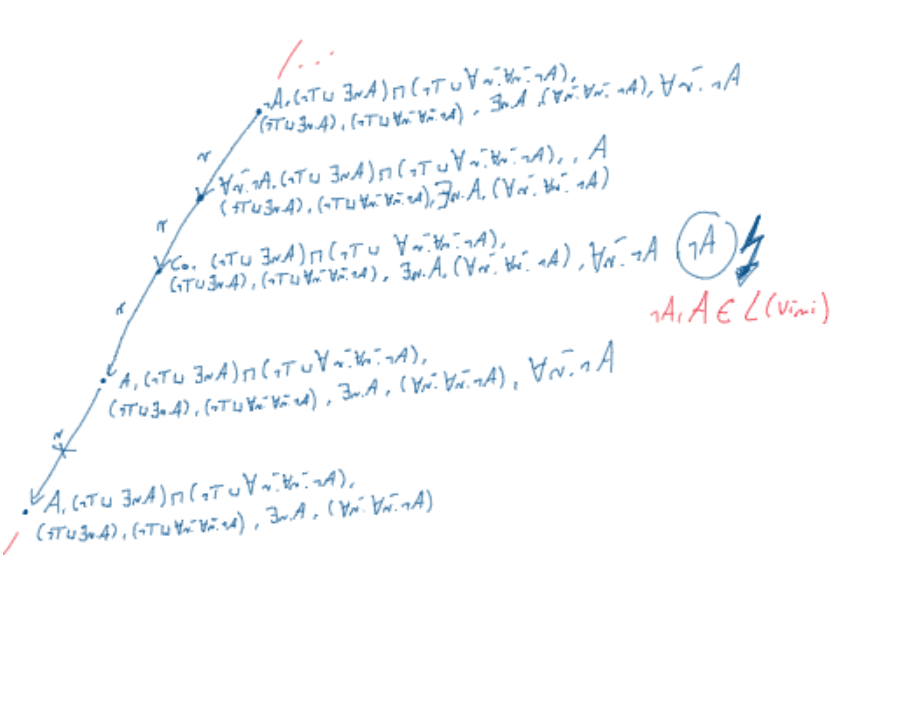
\includegraphics[width=\textwidth]{ab1}
    \caption{Aufgabe 5 - Tableau Algorithmus - Widerspruch wie im Text erklärt}
    \label{fig:meine-grafik}
\end{figure}
 \end{document}
 